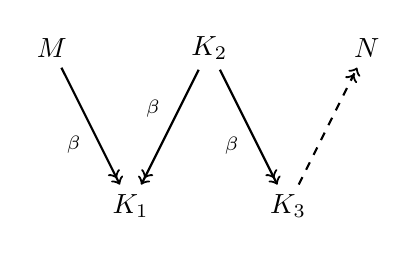
\begin{tikzpicture}[
    surj/.style={->>, line width=0.8pt},
    dashedsurj/.style={->>, dashed, line width=0.8pt}
    ]

    \node (M) at (0,2) {\(M\)};
    \node (K1) at (1,0) {\(K_1\)};
    \node (K2) at (2,2) {\(K_2\)};
    \node (K3) at (3,0) {\(K_3\)};
    \node (N) at (4,2) {\(N\)};
    
    \draw[surj] (M) -- node[below left]{\(\scriptstyle \beta\)} (K1);
    \draw[surj] (K2) -- node[above left]{\(\scriptstyle \beta\)} (K1);
    \draw[surj] (K2) -- node[below left]{\(\scriptstyle \beta\)} (K3);
    \draw[dashedsurj] (K3) -- (N);

\end{tikzpicture}